\section{Database Management}

A database is an efficient and well organized method of storing the statistics collected by the system. A MySQL database was selected for it's 
well documented use and easy integration into Python applications via the MySQLConnector class \cite{mysqlconnector}. A single database maintained on a machine on the same network as the nodes is used to store the statistics they transmit. The design of the system can be seen in Figure \ref{fig:erd} and Table \ref{table:entity_attributes}.

\begin{figure}[H]
    \centering
    \centering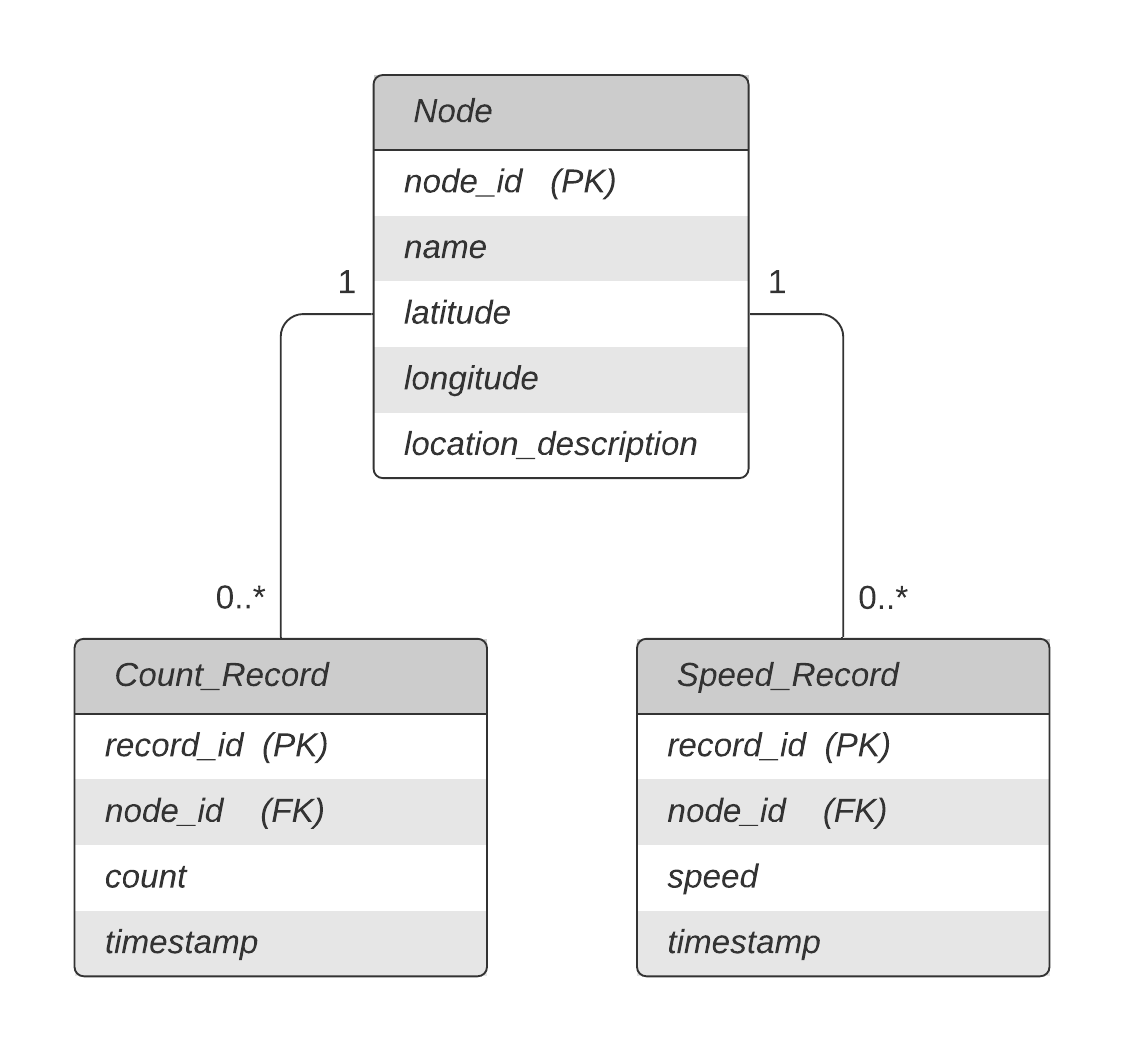
\includegraphics[width = 0.8\textwidth]{design/database/dragonfly_database_ERD}
    \caption{Entity Relationship Diagram of the system database.}
    \label{fig:erd}
  \end{figure}

\begin{table}
\def\arraystretch{1.5}
\begin{center}
\begin{singlespace}
    \begin{tabular}{|M{2.5cm}|M{2cm}|M{4cm}|M{3cm}|M{1cm}|} 
        \hline
        \textbf{Entity Name} & \textbf{Attributes} & \textbf{Description} & \textbf{Data Type} & \textbf{Null}\\
        \hline
        \multirow{5}{*}{Node} 
        & node id & A number that uniquely identifies the entity. & INT & N\\ \cline{2-5}
        & latitude & Latitude used to locate node. & DECIMAL(10,8) & N\\ \cline{2-5}
        & longitude & Longitude used to locate node. & DECIMAL(10,8) & N\\ \cline{2-5}
        & location description & A number that uniquely identifies the entity & VARCHAR(120) & Y\\
        \hhline{|=|=|=|=|=|}
        \multirow{5}{*}{Speed Record} 
        & record id & A number that uniquely identifies the entity. & INT & N\\ \cline{2-5}
        & node id & Unique node identifier linking record to its node. & INT & N\\ \cline{2-5}
        & speed & A single speed reading averaging vehicle speeds over 30 seconds. & DECIMAL(4,2) & N\\ \cline{2-5}
        & timestamp & Time stamp indicating when the speed reading began collecting data. & DATETIME & N\\
        \hhline{|=|=|=|=|=|}
        \multirow{5}{*}{Count Record} 
        & record id & A number that uniquely identifies the entity. & INT & N\\ \cline{2-5}
        & node id & Unique node identifier linking record to its node. & INT & N\\ \cline{2-5}
        & count & A single count reading for 30 seconds of traffic. & DECIMAL(4,2) & N\\ \cline{2-5}
        & timestamp & Time stamp indicating when the speed reading began collecting data. & DATETIME & N\\
        \hline
    \end{tabular}
\end{singlespace}
\end{center}
\caption{Attribute data for the system's database entities.}
\label{table:entity_attributes}
\end{table}